\documentclass[12pt,oneside,letterpaper]{article}
\usepackage{graphicx} % Required for inserting images
\usepackage{amsfonts}
\usepackage{amssymb}
\usepackage{hyperref}
\usepackage{listings}
\usepackage{tikz}
\usepackage{amsmath}
\usepackage{caption}
\usepackage[margin=0.6in]{geometry}
\usepackage{pdflscape}
\title{CARLA Leave-Over Documentation}
\author{Hunter White}
\date{April 2024}

\begin{document}
\maketitle
\newpage
\tableofcontents
\newpage
% NOTE: IF computer does not recognize joystick "Racing wheel" open Logitech Gaming software"


\section{Overview}
\label{sec:Overview}
This document is intended to serve as a resource for getting started with the "open-source driving simulator for autonomous driving research" known as Car Learning to Act \href{https://carla.org/}{CARLA}. It includes a description of CARLA, the steps taken to install and configure CARLA on both lab computers, and the scripts, terminal commands, and workflow for interacting with CARLA that may be useful. A significant effort is made to include solutions to errors that may be encountered during the installation and initialization processes, as well as links to StackOverflow/Linux Forums/CARLA Documentation pages that proved useful in the troubleshooting and error correction processes.
\section{Creating the Simulation Environment}

\subsection{Environment setup and package installation}
\subsubsection{Package and Environment Managers}
\label{subsec: Environment Managers}
\textbf{Definitely Review For Consistency}\\
\href{https://www.anaconda.com/}{Anaconda} is used as the package and environment manager. \href{https://www.anaconda.com/products/navigator}{Anaconda Navigator} vastly simplifies the package and environment management problem by providing a relatively simple, if a little bloated, graphical user interface for managing virtual environments, with shortcuts to launch common programs with the conda environment activated. This proved especially useful when initially exploring the best (read: easiest to integrate with existing machine learning research on GitHub) version of python and CARLA to work with. Most packages can be installed via conda or pip, although some require one or the other. A short comparison between conda and pip is given \href{https://www.anaconda.com/blog/understanding-conda-and-pip}{on the conda blog} Special care should be taken to install all possible packages with one installer and then the other if necessary, as conda does not communicate with pip and vice-versa. % Should probably find a better way to word this. 
A getting started guide for conda is available \href{https://docs.conda.io/projects/conda/en/latest/user-guide/getting-started.html}{here}.
When installing packages with conda, it will be useful to add the conda-forge channel. A guide on how to do that is provided \href{https://docs.conda.io/projects/conda/en/latest/user-guide/concepts/channels.html}{here}.
Note: Occasionally, updating conda before installing all desired packages will result in a deadlocked environment. Unfortunately, the only way to fix the environment is to delete it and reinstall all desired packages in a new environment. Generally, it is best to update conda before creating a new environment or starting a new project and avoid updating conda otherwise.
\\
\subsubsection{Required Packages}
\label{subsec:Requirements}
\textbf{Be sure to update pip and conda before creating a new environment and downloading packages for CARLA or the provided code.} \\
To run the provided code, the following packages and python version are/is necessary:
\begin{table}[h]
\centering
 \begin{tabular}{| c | c | c |}
 \hline
 Package & Version & requirements filepath \\
 \hline 
CARLA & 0.9.8 & N/A \\
 Python & 3.7.* & N/A \\
 numpy & 1.21.1 & (your-carla-filepath)/carla/PythonAPI/examples \\
 pygame & 2.1.2 & (your-carla-filepath)/carla/PythonAPI/examples \\
 matplotlib & * & (your-carla-filepath)/carla/PythonAPI/examples \\
 open3d & * & (your-carla-filepath)/carla/PythonAPI/examples \\
 pillow & 9.4.0 & (your-carla-filepath)/carla/PythonAPI/examples \\
 future & 0.18.3 & (your-carla-filepath)/carla/PythonAPI/examples \\
 networkx & * & (your-carla-filepath)/carla/PythonAPI/carla \\
 distro & * & (your-carla-filepath)/carla/PythonAPI/carla \\
 Shapely & 1.7.* & (your-carla-filepath)/carla/PythonAPI/carla \\
 psutil & * &  (your-carla-filepath)/carla/PythonAPI/util \\
 py-cpuinfo & * & (your-carla-filepath)/carla/PythonAPI/util \\
 python-tr & * & (your-carla-filepath)/carla/PythonAPI/util \\
 poetry & 1.3.2 & (your-repository-path)/requirements.txt \\
 \hline
 \end{tabular}
\caption{Required packages for CARLA, CARLA examples, and the provided code}
\label{table:RequirementsTable}
\end{table}

To install all of the above packages, open your prefered command line interface and activate your conda environment. You can then install the packages in either of the following ways:

\begin{enumerate}
\item(Option 1: Individually) All required packages can be installed by navigating to each \begin{verbatim} requirements.txt \end{verbatim} within your local copy of the \href{https://github.com/hrwhite21/RL_CARLA_ADAS}{GitHub Repository} and running the command \begin{verbatim} pip install -r requirements.txt \end{verbatim} or \begin{verbatim}conda install --yes --file requirements.txt \end{verbatim} in the command prompt with the desired conda environment activated.
\item(Option 2: Grouped) A single \begin{verbatim} requirements.txt \end{verbatim} file is provided for easier installation with pip. This is installed the same way as described in Option 1. Alternatively, the conda equivalent \begin{verbatim} <environment_name>.yml \end{verbatim} file is also provided. To install the \begin{verbatim} <environment_name>.yml \end{verbatim} file, use the command \begin{verbatim} conda env create -f <environment-name>.yml \end{verbatim} in the command prompt or terminal.
\item(Note on Poetry) Poetry is included as an alternate package manager, and was used by \href{https://github.com/idreesshaikh}{Idrees Razak} when creating the PPO agent and variational autoencoder that I used as a foundation. Poetry's main function in the repository is to download the legacy versions of PyTorch and CUDA that were used to train the PPO agent and VAE. To install these with Poetry, navigate to the Poetry folder using the command prompt or powershell, then run the command \begin{verbatim} poetry update \end{verbatim} As a disclaimer, I don't think this step is necessary if you would rather install the correct PyTorch and CUDA packages using pip or conda. The legacy versions can be found on the \href{https://pytorch.org/get-started/previous-versions/}{PyTorch website}
\end{enumerate} 

If you try option 2 and find that packages are missing, please try option 1.

\section{How to Download and Install CARLA}
\label{sec:CARLAInstall}
\textbf{NOTE: CARLA requires a dedicated GPU for with at least 6GB of VRAM. This excludes most consumer laptops.} More VRAM does not necessarily make CARLA run faster, but it does generally make CARLA more stable when adding large numbers of actors. CARLA also recommends having an addition GPU for any machine learning, although this is not necessary if your GPU has the capacity. (i.e. ~12 GB of VRAM and from a recent generation of Vulkan compatible GPUs)
CARLA is fairly easy to install, %and the process is nearly identical for Windows and Linux (Ubuntu). 
Because we do not need the additional functionality gained by building CARLA from source, we can follow the \href{https://carla.readthedocs.io/en/latest/start_quickstart/}{quick getting started guide.} \textbf{NOTE: There are different versions of documentation that correspond to each released version of CARLA.} Make sure you use the documentation version that corresponds to the CARLA version you intend to use. Be sure to make sure that pip and/or conda are up to date before creating the environment. \\


\section{Verifying CARLA installation}
\label{sec:verifyInstall}
CARLA provides a number of examples that are useful for checking that CARLA and its required packages were installed correctly. These provided examples are also useful for understanding the CARLA Python API, and give some ideas on how to structure code that will interact with CARLA. The \href{https://carla.readthedocs.io/en/latest/python_api/}{latest version of the Python API Reference} can be found here. 

\subsection{Opening a CARLA server instance: Windows}
\label{sec:CARLAserverwindows}
To open a carla instance on Windows, first open the terminal by pressing "ctrl+x" and selecting terminal. Depending on your windows preferences and configuration, this will open either a powershell instance or a command promptinstance. For our purposes, they are largely interchangeable, although powershell may be more familiar if you have previous experience. In your terminal, navigate to the CARLA folder by using the change directory function, abbreviated cd. 
\\
I have extracted CARLA to \begin{verbatim} C:\WindowsNoEditor \end{verbatim}.
\\
 \textbf{insert command line figure showing cd to carla directory.}
If you are having trouble navigating to your CARLA directory, you can copy the path to your directory by finding the directory in file explorer and  right clicking on the "TOP MIDDLE WINDOW THINGY?" and selecting copy address as text. You can then paste the address into your terminal after the call to change directory.
Alternatively, you can navigate through your files and directories by using a combination of ls, which lists the files and directories within the current directory, and cd. 

To start an instance of CARLA after navigating to the CARLA directory, simply run the command \begin{verbatim} .\CARLAUE4.exe \end{verbatim} in the terminal. A black window should pop up on the screen. After a few moments, the window should load to the default town for your version of CARLA. In CARLA 0.9.8, it should look like this:
\\ 
\textbf{Insert default carla window here for 0.9.8}

You can use the WASDQE keys to navigate the spectator camera around the default map. There's not much to see, as we haven't loaded in vehicles, pedestrians, etc. (a.k.a. "Actors"), but this will give you a feel for how smoothly CARLA runs on your device.

\subsection{running an example script}
To add in some actors, we will need to open an additional terminal window, and make sure the conda environment is activated. The easiest way to do this is to install the powershell/command prompt shortcut in anaconda navigator, or by typing conda activate <your CARLA environment name>. You will see the name of your environment in parenthesis in your terminal prompt if you have successfully activated your environment. Next, navigate to the Python API examples directory within your CARLA directory using the terminal window with your activated conda environment. the examples directory should have a path similar to :
\begin{verbatim}<your_carla_directory>\PythonAPI\.examples  \end{verbatim}

from here, running any of the example scripts should work. My personal favorite is \begin{verbatim} manual_control.py \end{verbatim}, which allows the user to manually control a vehicle using the keyboard. This example, and the corresponding \begin{verbatim} manual_control_steeringwheel.py \end{verbatim} , are also exceptionally useful for understanding how to integrate PyGame and outside control commands into a CARLA environment.
Experimenting with the example scripts is a great way to understand how to interact with CARLA and can serve as a great template for writing your own scripts. Other scripts included in the  \begin{verbatim}<your_carla_directory>\PythonAPI\.carla\agents\navigation  \end{verbatim} directory can be useful for understanding the basics of path planning and route creation.

\section{Driving Simulator Hardware}
The steering wheel and pedals have been modified from a \href{https://www.logitechg.com/en-sa/products/driving/driving-force-racing-wheel.941-000123.html}{Logitech G920 Driving Force Racing Wheel and Pedals for Xbox}.  These modifications and the manufactured base for the wheel and pedals were created by a previous senior design team. Their accompanying documentation can be found as a .zip file \href{https://alabama.box.com/s/ppm0j7ax0zvq7z98z6g3qv7kapbet37a}{here}. \textbf{NOTE: I have changed the microcontroller from the Atmel ATSAMC21N18A to an Arduino Uno Rev3}. I had issues understanding and using the Atmel microcontroller, but you are welcome to reintegrate it if you so desire. The rest of the user manual and parts lists/files are unchanged and are still valid. 

\subsection{Electrical Information}
The power for the driving system and its components (arduino, steering wheel, pedals, motors, motor controllers) is provided by several electrical connections.
\begin{enumerate}

\item(Steering Wheel and Pedals ) The steering wheel and pedals are connected to the alienware desktop computer via a USB connection. This connection allows the steering wheel and pedals to report changes in state to the computer, and it necessary for the steering wheel and pedals to be recognized by other programs. The displacement of the pedals is measured via potentiometers located at the base of the pedals, PICTURED HERE. A Picture of the USB connection can be found below. Power for the force feedback and calibration functionalities of the steering wheel is provided by the power adaptor. This connector must be plugged in initially, and can be power cycled to force the steering wheel to re-center. This connection must be UNPLUGGED prior to using the stepper motors, as the force feedback generated by the powered wheel is stronger than the torque applied by the stepper motor for the steering wheel. A picture of the power adapter is provided below.

\item(Arduino Uno) The Arduino Uno is intended to be powered with the USB-A to USB-B cable provided. This cable supplied the arduino with 5V, and also connects the desktop and arduino via serial connection. The serial port can be checked using the Arduino IDE. Connecting the Arduino to the computer is essential for actuating the stepper motors.

A PICTURE OF THE ARDUINO UNO IS PROVIDED BELOW.

\item(Stepper Motor Drivers) The stepper motor drivers used in this project are \href{https://www.amazon.com/SainSmart-Micro-Stepping-Stepper-Driver-ST-M5045/dp/B00DFSF9GE/ref=cm_cr_arp_d_product_top?ie=UTF8}{SainSmart ST-M5045 Microstepping Stepper Drivers}. These motor drivers accept 24-50VDC, can output up to 4.5A, and have numerous settings for microstepping, which is useful in reducing resonance (awful sounds) and torque-to-start in stepper motors. These drivers will need to be upgraded or changed to match more powerful or closed loop encoders.

\item(Stepper Motor - Pedals) The stepper motors used for the brake and accelerator pedals are \href{https://www.omc-stepperonline.com/nema-23-bipolar-3nm-425oz-in-4-2a-57x57x114mm-4-wires-stepper-motor-cnc-23hs45-4204s}{Nema 23 Bipolar 3Nm(425oz.in) 4.2A 57x57x113mm 4 Wires Stepper Motor CNC}. This motor can be driven with high voltages (generally - 10x-15x the rated voltage) without issues, and can operate exceptionally quickly without missing steps. These motors are likely fine for continued use, although they could be replaced with similar closed loop stepper motors for guaranteed tracking performance. This replacement would likely be necessary for increased performance and accuracy.
A PICTURE OF THESE MOTORS IS PROVIDED BELOW

\item(Stepper Motor - Steering Wheel) The stepper motor used to drive the steering wheel is an \href{https://www.automationdirect.com/adc/shopping/catalog/motion_control/stepper_systems/dual_shaft_and_encoder_stepper_motors/stp-mtr-23079d}{Automation Direct STP-MTR-23079D}. This motor is inadequate to drive the steering wheel at the speeds and acceleration required for this application without missing steps, even when driven at 48V. The motor may miss steps for two reasons: it does not produce enough torque to entirely overcome the rotational inertia of the steering wheel and itself, and it cannot be driven at a high enough voltage to overcome the effects of the inductance of its coils on its acceleration. The motor cannot be driven at a higher voltage without replacing the stepper driver (DETAILED IN NEXT SECTION), the power supply (FOLLOWING SECTION), and cannot be made to accept greater amperage, thus limiting its overall maximum torque. A replacement motor should be sized according to the maximum torque required to counter the rotational inertia of the steering wheel and motor at maximum speed, with a caution margin of 10-20 percent. There are numerous other ways to size a stepper motor, and a simple guide can be found in \href{https://forum.arduino.cc/t/stepper-motor-basics/275223}{this forum post}. Alternate solutions may include a stepper brake, an encoder mechanism, and a resized motor.

\item(Power Supply/Supplies) Originally, the stepper motors and motor drivers were powered by a single 24V 15A DC power supply, similar to \href{https://www.amazon.com/Switching-SJHPRMXF-Universal-Regulated-Transformer/dp/B0BWC8J2HY/ref=sr_1_4?crid=2KFHB4ZPW918C&dib=eyJ2IjoiMSJ9.FPK3xtReWIHdljtMiM5tJdXhBQ5q_-IO-pflt5CI00iFDB9iYGMc79Ty_FO0dvSjdtl0D0Zih9khd_51xjQamVo7iaApGN1fatpqVmezqN7-BDClRtcv_gsEr8ofznzE0bb5uG-HI-YOc7R0-aT_jQXBuObvvQguQbhkOHwR9Rz7JSEfk6LCDIEusBev-jj4meyV8GGQBtdx2AE4DfrnhkPKcfrdVDSSCgHEC-I6Ccjzjrr8_a77e0xSFJ9ziQedmuPHjgInys8orLajkbVt0rwaIr624xeHIuU9LhTWBNQ.29UMZP6yEU8jGo2FBFcXFL1GxivPtxQHOTDhLT26qvg&}{this generic amazon posting}. This primary power supply was connected in series with another 24V 15A power supply following\href{https://www.youtube.com/watch?v=jbzb66dCbOc}{this YouTube video}. \textbf{PLEASE BE AWARE: this is generally a bad idea, for numerous reasons. Improperly sized wires, undersized power supply components, and numerous electrical phenomena beyond my comprehension render this a dangerous, hacky solution at best. This should be replaced by a PROPER 48V or 60V power supply at an appropriateamperage rating as soon as possible.}

\end{enumerate}
\begin{landscape}
\subsection{Wiring Diagram}
\begin{figure}[h!]
\centering
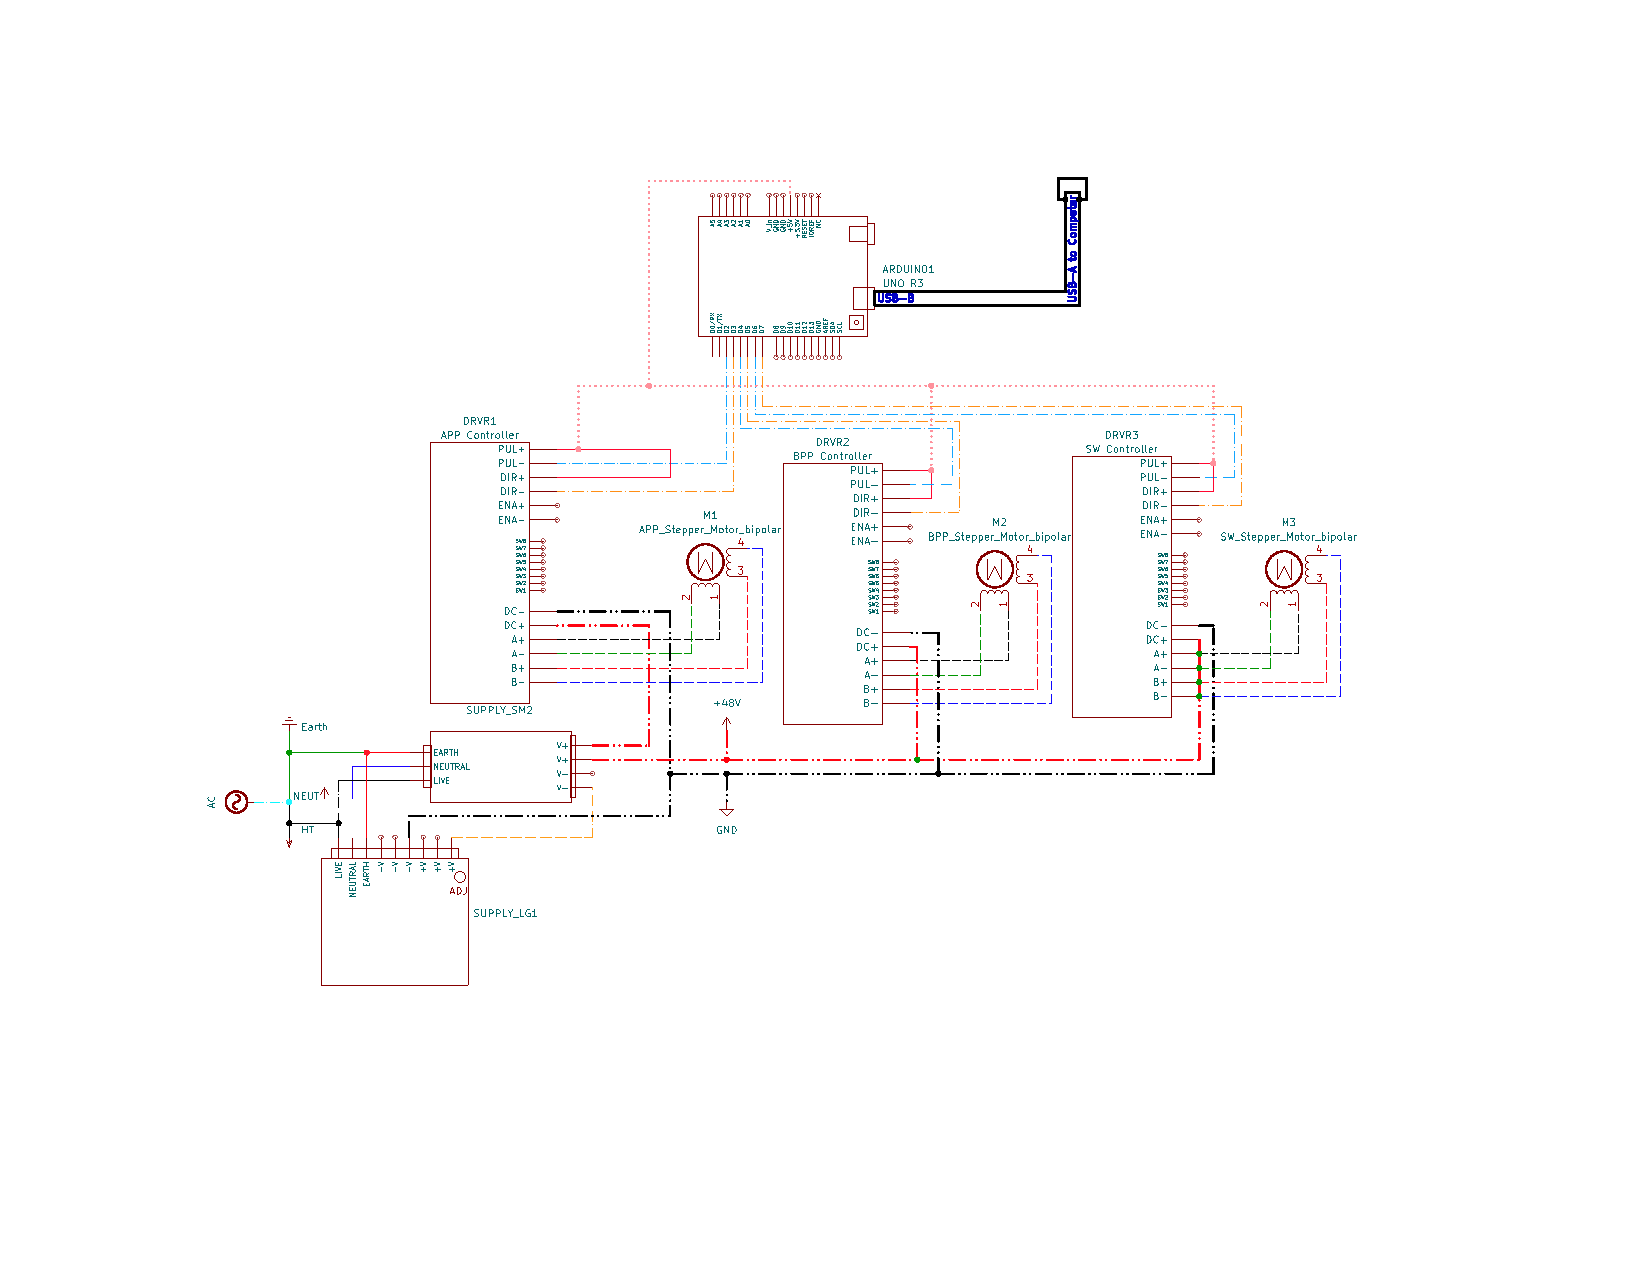
\includegraphics[width=\textwidth, trim=3.5cm 4.5cm 5.0cm 2.5cm, clip,scale=1.5]{Print Schematic_R7.pdf}
\caption{Complete wiring diagram for the fully connected electrical system. \textbf{Note:} The colors and sizing of wires may not match, and all connections should be verified before testing circuit functionality}
\end{figure}
\end{landscape}
\newpage
\subsection{Arduino Configuration and Code Walkthrough}
The Arduino code for interfacing between Python, CARLA, and the Driving Simulator can be found \href{https://github.com/hrwhite21/DriverlessDIL/blob/main/PythonToMotor/PythonToMotor.ino}{here}. In its current implementation, the bits corresponding to the pins for the step and direction function are directly manipulated (set to 1, 0, or -1) instead of being changed via the traditional DigitalRead() and DigitalWrite() functions. This reduces the amount of time required to change the pins by a significant amount. Unfortunately, this makes the code VERY difficult to read and debug. A more understandable version can be found in the \href{https://tinyurl.com/2s4kpnuv}{the commit history for the aruino ".ino" file.}
\\
To give a quick overview: The script begins by defining the pins connecting the arduino and the motor controllers. It is important to make sure that these pins are correct and the connections are stable. Max displacement values are assigned based on an initial calibration. The max displacement values should be re-defined when changing the length of string attaching the pedals to the motors, the settings on the motor controllers, or after any catastrophic failure type event. The pins as outputsand given initial states in the setup() loop. Serial communication is opened on the COM port corresponding to the Arduino board at the specified baud rate. This serial communication interface is also how python will interact with the arduino. The loop and accompanying functions generally do the following: 
\begin{enumerate}
\item As a debug function : Print the current displacement of the wheel and pedals if it has been longer than "printInterval" milliseconds since the last check. This is not guaranteed to be the true position, and the system should be \hyperref[sec:Calibration]{recalibrated to zero} before interfacing with CARLA/Python.
\item Checks if there is information waiting in the input buffer on the serial port corresponding to the Arduino Uno. 
\item If there is data available on the buffer, read the buffer until the newline character, Otherwise, return to (1)
\item Parse the data returned: seperate the read data into 3 values, seperated by a comma.
\item Constrain the returned values between and their respective minimum and maximum values
\item Check the current state of each direction pin, and change it if necessary.
\item While any of the [APP,BPP,SW] are not equal to the desired position, pulse the corresponding stepPins until all [APP,BPP,SW] are at desired position
\item Return to (1) 
\end{enumerate}

This loop generally runs very fast because it directly accesses the arduino pins, and does not rely on slower digitalRead and digitalWrite functions. This does make the arduino code difficult to understand and debug. The response of the motor to a commanded position is limited by a combination of factors, such as the voltage and amperage supplied to the motor, the minimum pulse width of the motor controller, and the rotational inertia of the motor. Setting delayMicros() too low without adjusting the degree of microstepping on the motor controller results in the motor "missing steps" and producing awful sounds. The most recent settings for the motor controllers are provided in the table: 

\begin{table}[h]
\centering
 \begin{tabular}{| c | c | c | c|}
 \hline
 Switch Number & APP Controller & BPP Controller & SW Controller \\
 \hline 
 Switch 1 & OFF & OFF  & OFF \\
 Switch 2 & OFF & OFF & OFF \\
 Switch 3 & OFF & OFF & OFF \\
 Switch 4 & ON & ON & ON \\
 Switch 5 & ON & ON & ON \\
 Switch 6 & ON & ON & ON \\
 Switch 7 & OFF& OFF & OFF \\
 Switch 8 & ON & ON & ON \\

 \hline
 \end{tabular}
 \caption{Stepper Driver Board Settings and Configuration}
 \label{table:StepperSettings}
\end{table}

\label{table: Most Recent Settings for Motor Controllers}

\subsection{Debugging and Troubleshooting Tips}

Problem: The steering wheel and pedals are not recognized by the computer. \\
Tip: Ensure that the USB for the wheel and pedals is plugged into the computer. Plug in the power cable (2 prong) for the wheel and pedals. In windowns, search for and open the program "Logitech Gaming Software". The steering wheel and pedals should be visible as two icons, and the wheel should have completed a calibration by rotating back and forth until settling in a central position. The act of unplugging and plugging in the USB and Power cable connections should also recalibrate the wheel to zero. \label{poi:Calibration} \\

Problem: One or multiple stepper motors "steps" even when the arduino is not commanding a step. \\
Tip: Make sure that the wires connecting the arduino and the stepper motor drivers are not contacting the stepper motors themselves. The stepper motors are constantly energized when the power supply/supplies are connected to AC power, and because of the internal construction of the motors, they can induce voltages in surrounding wires. If the steppers are in contact with a "step" wire, then they may generate "ghost commands".\\

Problem: The wiring diagram does not match "XYZ" component. \\
Tip: The wiring diagram was created using KiCAD 8.0, which offers a near-limitless number of color options when creating wire diagrams, but does not include representation for the stepper driver boards or the arduino uno. In reality, only some of these colors used in the wiring diagram are readily available for use. Every effort has been made to balance readibility of the wiring diagram with fidelity to the actual hardware and connections.  As always, cross-referencing the supplier data sheets, google, and using a multimeter to double check that components are receiving the correct voltage and signals will be very helpful troublehsooting steps.\\

\textbf{additional problems to come, surely}

\section{Code and Software}
This section will cover the included code files and any other software included in the box/GitHub links.

\subsection{Included Files}
Several files are included in this project, separated into various folders. Each file handles a specific task during the simulation. The folders and files are listed below, including a short description of their purpose.
\begin{itemize}
\item FILE -- Python-Uno-DIL-Interface.ino : This file initializes the serial communication port between the arduino and the computer, and contains the logic that actuates the stepper motors to a specific position. This file can also be used as a standalone way to test the functionality of the arduino and stepper motor system, and it most often used during debugging and calibration.
\item FOLDER -- autoencoder : This folder contains all of the python files associated with creating and using the variational autoencoder. Variational Autoencoders (VAEs) are a type of generative model in machine learning, introduced by Kingma and Welling in 2013. VAEs are designed to learn latent representations of input data that can be used to generate new, similar data. Generally, autoencoders are used as feature extractors in reinforcement learning, compressing a complex, high-dimensional observation space into a lower-dimension latent space. Lower dimensional representations are generally easier to learn, and using a VAE can sometimes reduce training time and improve agent robustness to unseen scenarios. For a rather intuitive-yet-complete explanation of variational autoencoders, see \href{https://towardsdatascience.com/understanding-variational-autoencoders-vaes-f70510919f73}{this post by Joseph and Baptiste Rocca}. Additional readings are available \href{https://www.cs.toronto.edu/~rgrosse/courses/csc421_2019/slides/lec17.pdf}{from University of Toronto} and \href{https://towardsdatascience.com/intuitively-understanding-variational-autoencoders-1bfe67eb5daf}{Irhum Shafkat}
\item FOLDER -- checkpoints : This folder contains all of the checkpoints for the proximal policy optimization (PPO) machine learning agent on both Town07 and Town02. The checkpoints are made every 100 episodes, and serve as a training log for the agent. These are useful for evaluating how well an agent was performing at different stages of training, but DO NOT contain the actual trained agents.
\item FOLDER -- copy\_of\_PythonAPI\_for\_reference : This folder is a copy of the PythonAPI folder included in a CARLA installation. The files in these folders are extremely useful for learning how to interact with CARLA via python, and also include helpful functions for creating routes, changing weather, and adding sensors and actors to a CARLA instance. 
\item FOLDER -- networks - This folder contains the python files that define the structure and functions associated with the PPO agent. These files can be useful for understanding the general structure of the agent and for understanding how to implement the underlying probability distrubutions using PyTorch. The agent used in the training/evaluation simulations is generated from these files.
\item FOLDER -- preTrained\_models : This folder contains the trained agents associated with the files found in the checkpoint folder. Loading these agents in allows one to reproduce an agent at the corresponding stage of training.
\item FOLDER -- Simulation : This folder contains all the scripts which define sensor settings, connect python to CARLA, create the machine learning environment, and populate the CARLA simulation with additional actors. The files are relatively self-explanatory, with environemnt.py being the exception.
\item FILE -- continuous\_driver.py : This file is the equivalent of main.py. It contains all of the information regarding user argument tags, and calls all other necessary functions to connect to a CARLA instance, change the town and weather, create the machine learning agent, and spawn the actor for the machine learning agent to control. This file is also repsonsible for calling the functions to create checkpoints and save models during training.
\item FILE -- parameters.py : This file contains the information on all machine learning related parameters outside of network structure.
\item File -- pygame\_test\_joystick.py : This file is important in verifying the functionality of the steering wheel and pedals in python. This script creates a debug display that reports the values for each of the buttons, axes, and directional pads for the steering wheel, pedals, and any other controller connected to the computer that is not a mouse and keyboard. The most common uses of this script are to verify that the steering wheel has returned to a zero position before continuing with training or evaluation.
\item FILE -- wheel\_config.ini : This file contains the mapping between pygame and the logitech wheel and pedals. This will need to be changed if using a different controller.

\end{itemize}

\subsection{Primer on PPO}

Proximal Policy Optimization (PPO) is a popular reinforcement learning (RL) algorithm designed to train agents to make decisions by interacting with an environment to maximize cumulative rewards. PPO stands out because it strikes a balance between performance and simplicity. PPO is an actor-critic based  policy gradient method. Policy gradient methods optimize the policy directly, as opposed to value-based methods which optimize the value function. In simpler terms, a policy gradient method adjusts the policy (the agent’s behavior) based on feedback from the environment. PPO can be used in both discrete and continous action spaces, which makes it especially versatile - previous implementations of PPO in the fields of robotics and game playing have yielded incredible results. \\

\subsection{Key Concepts and Equations}
\begin{itemize} 
\item Policy -  is like a set of rules or a strategy that an agent follows to decide what action to take in different situations. Think of it as the agent's decision-making guide. Policies fall into two categories: Deterministic and Stochastic. Deterministic policies \textbf{always} take the same action given the same conditions. Stochastic policies take an action based on probabilities, and may \textbf{not always} take the same action given the same conditions. A policy is represented symbolically as $\pi_{\theta}$, "the policy parameterized by $\theta$. The probability of taking action $a$ given a state $s$ according to the policy $\pi_{\theta}$ is represented as $\pi_{\theta} (a | s )$, and is a value between 0 and 1.
\item Value Function -  is a measure that helps the agent understand how good it is to be in a particular situation or state. It gives an estimate of the expected future rewards an agent can obtain starting from that state, following a certain policy. It is important to note that the value function is based on a particular policy, meaning it depends on the strategy the agent is following to decide its actions. Value functions fall into two categories with two distinct representations. The state-value function, represented by $V^{\pi}(s)$ gives the expected reward starting from state $s$ and following the policy $\pi$. It answers the question: "How good is it to be in this state?". The action-value function, represented by $Q ( s,a )$, gives the expected reward for taking action $a$ in state $s$ and then following the policy. It answers the question: "How good is it to take this action in this state?"
\item Surrogate Objective Functions - A surrogate objective function is an approximation of the true objective function that is easier to optimize. It serves as a proxy for the actual objective, capturing its essential characteristics while being more manageable computationally. In PPO, the surrogate objective function is designed to prevent large updates to the policy, which can destabilize training. The main surrogate objective used in PPO is based on the probability ratio between the new and old policies, combined with a clipping mechanism. The clipped surrogate objective function in PPO is defined as : \(L^{\text{CLIP}}(\theta) = \mathbb{E}_t \left[ \min \left( r_\theta(s_t, a_t) \hat{A}_t, \ \text{clip}(r_\theta(s_t, a_t), 1 - \epsilon, 1 + \epsilon) \hat{A}_t \right) \right] \), where : \\
\begin{itemize} 
\item $(r_\theta(s_t, a_t)$ is the probability ratio between the new and old policies for taking action $a_t$ given state $s_t$, or more simply : \( r_\theta(s_t, a_t) = \frac{\pi_\theta(a_t \mid s_t)}{\pi_{\theta_{\text{old}}}(a_t \mid s_t)} \). 
\item \( \hat{A}_t \) is the estimate of the advantage function : \( A^\pi(s, a) = Q^\pi(s, a) - V^\pi(s) \).  The advantage function measures how much better taking a particular action $a$ in state $s$ is compared to the average action in that state, under policy $\pi$. The advantage function can be estimated using various methods. One common method is Generalized Advantage Estimation (GAE), which balances bias and variance in the advantage estimates.
\item $\varepsilon$ is a hyperparamter that controls the clipping range. The clipping mechanism ensures that the updates to the policy do not deviate too much from the old policy by clipping the probability ratio $r_\theta(s_t, a_t)$ to be within  \( [1 - \varepsilon, 1 + \varepsilon]\). This prevents excessively large policy updates that could destabilize training.
\end{itemize}
\item The Generalized Advantage Estimation (GAE) is calculated as \( \hat{A}_t = \delta_t + (\gamma \lambda) \delta_{t+1} + (\gamma \lambda)^2 \delta_{t+2} + \ldots \)

\item The Temporal Difference (TD) error measures the discrepancy or difference between the predicted value of a state and the actual received reward at a particular time step. The TD error at time step $t$ , denoted as $\delta_t$, is defined as: \( \delta_t = r_t + \gamma V(s_{t+1}) - V(s_t) \). TD error is a measure of how well the agent's value function aligns with the observed outcomes in the environment.
\begin{itemize}
\item $r_t$ is the reward received after taking action $a_t$ in state $s_t$, and is defined by the reward function.
\item $\gamma$  is the discount factor, a value between 0 and 1 that discounts future rewards. $\gamma$ determines the importance of future rewards relative to immediate rewards.
\item and $V(s_t) \text{ and } V(s_{t + 1}) $ follow the definitions of state-value functions above.
\end{itemize}
\end{itemize}
\subsection{Goal of Project}
The goal of this project is to develop a reinforcement learning (RL) agent
% specifically using Proximal Policy Optimization (PPO),  NOT SURE About this line
to autonomously drive a vehicle within the CARLA simulation environment. The agent should effectively navigate urban and rural traffic scenarios, obey simple traffic rules, and be able to maintain a reasonable driving speed. The RL agent should process a visual input, either from CARLA or from a webcam directed at the screen, as well as vehicle telematic information, and output a corresponding tuple of (steering action, acceleration action, braking action).
\subsection{Training and Environment Setup}
The RL agent is implemented in Python 3.7.*, and utilizes the packages listed in \hyperlink{table:RequirementsTable}{requirements table}. Simulations and trainings were run on a system using an Nvidia Titan X, a 4-core Intel i7, and 32 GB of DDR4. The backbone of the training and implementation was adapted from \href{https://github.com/idreesshaikh/Autonomous-Driving-in-Carla-using-Deep-Reinforcement-Learning/tree/main}{this GitHub repository}, available under the MIT License. For compatability reasons, CARLA 0.9.8 with additional maps is used for training and evaluation. \\
The PPO Agent is composed of an actor network and a critic network. These networks are constructed of 3 fully-connected layers, with 500 , 300, and 100 nodes, each with a hyperbolic tangent activation function. The output layer of the actor network contains $a_{dim}$ nodes, corresponding to the size of the action space, and uses a $\tanh$ activation function. For this project, $a_{dim} = 3; \text{a tuple of (steer, throttle, brake)} $. The output layer of the critic network contains a single node, which represents an estimation of the state-value function. This layer contains no activation function. \\
The input to each network consists of the output of the VAE ([120,1]) and the following external features: current vehicle speed, previous steer action, current throttle/accelerator pedal position value, distance to the road center, and angular deviation from intended trajectory. \textbf{The Following Figure is included as a reference}:

A simulation may be terminated for violating the following reasons: \\
\begin{itemize}
\item the vehicle has a deviation greater than 3 meters from the center of the lane
\item the vehicle has a speed less than 1.0 km/hr after the first 10 simulated seconds have elapsed
\item the vehicle collides with the environment or another actor (vehicle, pedestrian, etc.)
\item the vehicle travels at a speed greater than the set maximum speed
\item the vehicle exceeds the maximum number of timesteps per simulation
\item the vehicle successfully completes its route
\end{itemize}

\subsection{State and Action Spaces}
The state space of the agent consists of the encoded result of the VAE, plus the five external features mentioned above. The action space consists of the tuple (steer, throttle, brake), with the values being continuous and bounded by the sets $\left([-1,1],[0,1],[0,1]\right)$.

\subsection{Reward Structure}
To encourage the RL agent to learn appropriate traffic behaviors, the following reward structure is used:
\[ \alpha_{reward}= \begin{cases}
1- | \frac{\alpha_{\text{deviation}}}{\alpha_{\text{max deviation}}} | & \alpha_{\text{deviation}} < \alpha_{\text{max deviation}} \\
0 & \text{otherwise}
\end{cases}
\]

\[ R = \begin{cases}
\frac{v}{v_{min}} * (1- d_{center} * \alpha_{reward}  & v < v_{min} \\
(1- d_{center} * \alpha_{reward}  & v_{min} \leq v <v_{target} \\
\left(1 - \frac{v - v_{target}}{v_{max} - v_{target}} \right) * (1- d_{center} * \alpha_{reward} & v \geq v_{target} \\
-10 & \text{Upon Constraint Violation}
\end{cases}
\]

% TODO:
% Implement all figures previously discussed.
% Rewrite first 3 Sections
% Include Figure for VAE
% Include Figure describing Waypoints and additional state features
% Include links to .mp4 of vehicle driving successfully?
% Improve Code Comments


\end{document}

